\documentclass[a4paper, table]{article}


% Loads in the preamble 
% Useful packages, sorted so packages of similar functionality are grouped together. Not all are essential to make the document work, however an effort was made to make this list as minimalistic as possible. Feel free to add your own!

% Essential for making this template work are graphicx, float, tabularx, tabu, tocbibind, titlesec, fancyhdr, xcolor and tikz. 

% Not essential, but you will have to debug the document a little bit when removing them are amsmath, amsthm, amssymb, amsfonts, caption, subcaption, appendix, enumitem, hyperref and cleveref.

% inputenc, lipsum, booktabs, geometry and microtype are not required, but nice to have.

\usepackage{todonotes}

\usepackage[utf8]{inputenc} % Allows the use of some special characters
\usepackage{amsmath, amsthm, amssymb, amsfonts} % Nicer mathematical typesetting
\usepackage{lipsum} % Creates dummy text lorem ipsum to showcase typsetting 

\usepackage{graphicx} % Allows the use of \begin{figure} and \includegraphics
\usepackage{float} % Useful for specifying the location of a figure ([H] for ex.)
\usepackage{caption} % Adds additional customization for (figure) captions
\usepackage{subcaption} % Needed to create sub-figures

\usepackage{tabularx} % Adds additional customization for tables
\usepackage{tabu} % Adds additional customization for tables
\usepackage{booktabs} % For generally nicer looking tables

\usepackage[nottoc,numbib]{tocbibind} % Automatically adds bibliography to ToC
\usepackage[margin = 2.5cm]{geometry} % Allows for custom (wider) margins
\usepackage{microtype} % Slightly loosens margin restrictions for nicer spacing  
\usepackage{titlesec} % Used to create custom section and subsection titles
\usepackage{titletoc} % Used to create a custom ToC
\usepackage{appendix} % Any chapter after \appendix is given a letter as index
\usepackage{fancyhdr} % Adds customization for headers and footers
\usepackage[shortlabels]{enumitem} % Adds additional customization for itemize. 

\usepackage{hyperref} % Allows links and makes references and the ToC clickable
\usepackage[noabbrev, capitalise]{cleveref} % Easier referencing using \cref{<label>} instead of \ref{}

\usepackage{xcolor} % Predefines additional colors and allows user defined colors

\usepackage{tikz} % Useful for drawing images, used for creating the frontpage
\usetikzlibrary{positioning} % Additional library for relative positioning 
\usetikzlibrary{calc} % Additional library for calculating within tikz

% Defines a command used by tikz to calculate some coordinates for the front-page
\makeatletter
\newcommand{\gettikzxy}[3]{%
  \tikz@scan@one@point\pgfutil@firstofone#1\relax
  \edef#2{\the\pgf@x}%
  \edef#3{\the\pgf@y}%
}
\makeatother












% Loads in user defined settings
% Give your report a title
\newcommand\reporttitle{Lab Report TP Micro 332}

% Insert course code, name, quartile number and year (or any other subtitle)
\newcommand\reportsubtitle{\noindent
MICRO-332 \\
Microfabrication Practicals \\
MT-BA 2023-2024 \\
}

% Add your group number (for DBL) or any other text.
\newcommand\groupnumber{
\Large\textbf{Group \#32}
}   

% Insert authors and student numbers here
\newcommand\reportauthors{\noindent
Maxime Nourry & 314936 \\
Yann Thome & 329311 \\
Viktor Ellevseth & 376610 \\
Luka Vecerina & 299871 \\
Loïc Delineau & 296451 
}

% Add the name of your tutor (for DBL) or any other text.
\newcommand\grouptutor{
\textbf{\textcolor{Tue-red}{Professor:}} Jürgen Brugger \\
\textbf{\textcolor{Tue-red}{Tutor:}} Abdeljalil Sayah \\
}

\newcommand\practicaldates{\noindent
TP \#1 & 13th of November 2023 \\
TP \#2 & 4th of December 2023 \\
TP \#3 & 4th of December 2023 \\
TP \#4 & 11th of December 2023 \\
TP \#5 & 5th of December 2023 \\
TP \#6 & 18th of December 2023 \\
TP \#7 & 19th of December 2023 \\
}

% Date and location (default: current date and Eindhoven)
\newcommand\placeanddate{
Ecublens, \today
}

% Define Tue-red (color of the EPFL logo). Can be changed to drastically change the look of the template
\definecolor{Tue-red}{RGB}{255, 0, 0}

% All of the following code can be removed to be left with (close to) default LaTeX behaviour. 

% Sets up hyperlinks in the document to be colored
\hypersetup{
    colorlinks=true,
    linkcolor=Tue-red,
    urlcolor=Tue-red,
    citecolor = Tue-red
    }
\urlstyle{same} % Defines settings for link and reference formatting


% Change bullet style for level 1, 2 and 3 respectively for itemize
\renewcommand{\labelitemi}{\scriptsize\textcolor{Tue-red}{$\blacksquare$}}% level 1
\renewcommand{\labelitemii}{\scriptsize\textcolor{Tue-red}{$\square$}}% level 2
\renewcommand{\labelitemiii}{\textcolor{Tue-red}{$\circ$}}% level 3

% \renewcommand{\labelitemi}{\small\textcolor{Tue-red}{\ding{70}}} % level 1
% \renewcommand{\labelitemii}{\small\textcolor{Tue-red}{\ding{71}}}% level 2
% \renewcommand{\labelitemiii}{\tiny\textcolor{Tue-red}{\ding{71}}}% level 3

% Change bullet style for level 1, 2 and 3 respectively for enumerate
\renewcommand{\labelenumi}{\textbf{\textcolor{Tue-red}{\arabic*.}}}% level 1
\renewcommand{\labelenumii}{\textbf{\textcolor{Tue-red}{[\alph*]}}}% level 2
\renewcommand{\labelenumiii}{\textbf{\textcolor{Tue-red}{\roman*.}}}% level 3

% Have reference labels be linked to section (section 3 will have fig. 3.1 etc.)
\counterwithin{equation}{section} % For equations
\counterwithin{figure}{section} % For figures
\counterwithin{table}{section} % For tables

% Creates a beautiful header/footer
\pagestyle{fancy}
\lhead{
\includegraphics[height = 20pt]{epfl-clean.png}}
\rhead{\reporttitle}
\renewcommand{\footrulewidth}{0.4pt}
\cfoot{Page \thepage}

% Formats section, subsection and subsubsection titles respectively 
\titleformat{\section}{\sffamily\color{Tue-red}\Large\bfseries}{\thesection\enskip\color{gray}\textbar\enskip}{0cm}{} % Formats section titles

\titleformat{\subsection}{\sffamily\color{Tue-red}\large\bfseries}{\thesubsection\enskip\color{gray}\textbar\enskip}{0cm}{} % Formats subsection titles

\titleformat{\subsubsection}{\sffamily\color{Tue-red}\bfseries}{\thesubsubsection\enskip\color{gray}\textbar\enskip}{0cm}{} % Formats subsubsection titles

% Formats captions
\DeclareCaptionFont{Tue-red}{\color{Tue-red}}
\captionsetup{labelfont={Tue-red,bf}}

 % Changes font to mlmodern
\usepackage{mlmodern}

% Removes indent when starting a new paragraph
\setlength\parindent{0pt}

% Limits the ToC to sections and subsections (no subsubsec.)
\setcounter{tocdepth}{2}




















\begin{document}


















% Inserts the front page
\begin{titlepage}

\centering

\begin{tikzpicture}

\node[inner sep=0pt] (logo) at (0,0){
    
\includegraphics[width= .25\textwidth]{epfl-titlepage.png}};
    
\node[text width = 0.5\textwidth, right = of logo](title){\sffamily\huge\reporttitle};

\node[text width = 0.5\textwidth, yshift = 0.75cm, below = of title](subtitle){\sffamily\Large \reportsubtitle};

\gettikzxy{(subtitle.south)}{\sffamily\subtitlex}{\subtitley}
\gettikzxy{(title.north)}{\titlex}{\titley}
\draw[line width=1mm, Tue-red]($(logo.east)!0.5!(title.west)$) +(0,\subtitley) -- +(0,\titley);

\end{tikzpicture}
\vspace{1cm}

% table for group members -------------
\sffamily\groupnumber

\begin{table}[H]
    \centering
    \sffamily
    \large
    \begin{tabu} to 0.8\linewidth {cc}
        \textbf{Full Name} & \textbf{SCIPER}\\
        \hline
        \sffamily\reportauthors
        \end{tabu}
\end{table}


\vspace{0.3cm}

\sffamily \grouptutor

\vspace{0.3cm}

% table for dates ----------------
\begin{table}[H]
    \centering
    \sffamily
    \large
    \begin{tabu} to 0.8\linewidth {cc}
        \textbf{Lab Number} & \textbf{Date}\\
        \hline
        \sffamily\practicaldates
    \end{tabu}
\end{table}



\tikz[remember picture,overlay]\node[anchor=south,inner sep=0pt] at (current page.south) {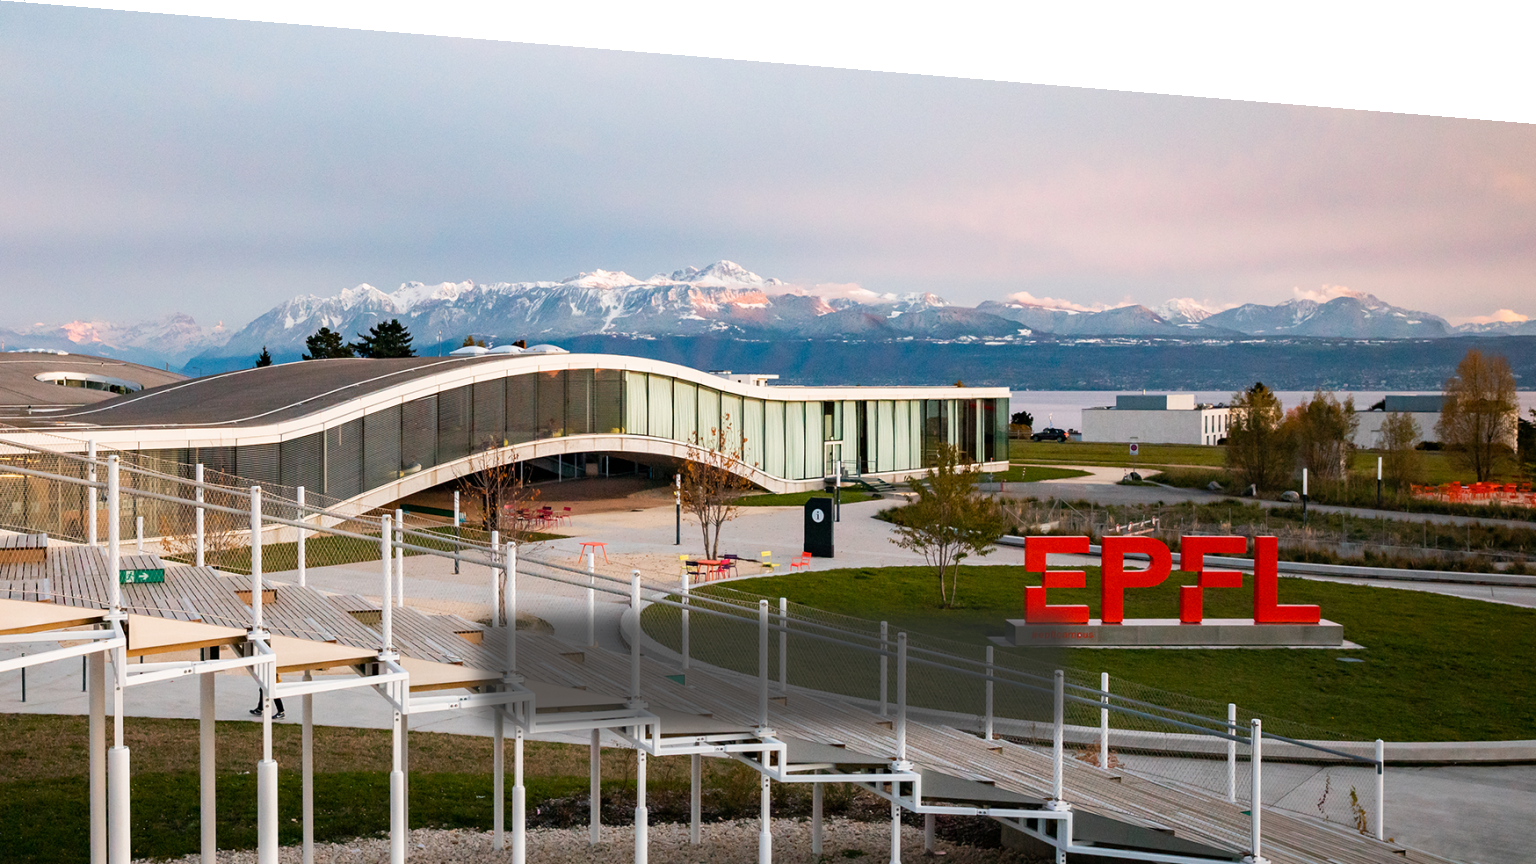
\includegraphics[width=\paperwidth]{epfl-landscape.png}};

\mbox{}
\vfill
\sffamily \Large \textcolor{white}{\placeanddate} \\



\end{titlepage}
\newpage



















% Generates a ToC without page number
{\hypersetup{linkcolor=black} % Keeps the ToC black even with non-black linkcolor
\tableofcontents\thispagestyle{empty}}
\newpage














% Insert (Z. Template) section
\section{Template Section}
\label{sec:Template}       % use below command to reference this section
                           % \cref{sec:Template}

% =========================================================
%                        SECTIONS 
% =========================================================
\subsection{This is a subsection}
    \subsubsection{This is a subsubsection}
    This is text.

% =========================================================
%                  GENERAL FORMATTING
% =========================================================
\subsection{General formatting}
Firstly, the document uses the font mlmodern, using no indent for new paragraphs and commonly uses the color \textcolor{Tue-red}{Tue-red}.
The \texttt{hyperref} package is responsible for highlighting and formatting references like figures and tables. For example \cref{table: style 1} or \cref{fig: three images}. It also works for citations \cite{texbook}. Note how figure numbers are numbered according to the format \texttt{<chapter number>.<figure number>}.\\

% =========================================================
%                       Bulleted Lists 
% =========================================================
\subsection{Bulleted Lists}
Bullet lists are also changed globally, for a maximum of 3 levels:

\begin{itemize}
    \item Item 1
    \begin{itemize}
        \item subitem 1
        \begin{itemize}
            \item subsubitem 1
            \item subsubitem 2
        \end{itemize}
    \end{itemize}
\end{itemize}

Similarly numbered lists are also changed document wide:

\begin{enumerate}
    \item Item 1
    \item Item 2
    \begin{enumerate}
        \item subitem 1
        \begin{enumerate}
            \item subsubitem 1
        \end{enumerate}
    \end{enumerate}
\end{enumerate}


% =========================================================
%                         TABLES 
% =========================================================
\subsection{Tables}
The following table, \cref{table: style 1}, shows a possible format for tables in this document. Alternatively, one can also use the black and white version of this, shown in \cref{table: style 2}. Note that caption labels are in the format \textbf{\textcolor{Tue-red}{Table x.y:} }

% Table 1 (style 1) ---------------------------
\begin{table}[ht]
    \rowcolors{2}{Tue-red!10}{white}
    \centering
    \caption{A table without vertical lines.}
    \begin{tabular}[t]{ccccc}
        \toprule
        \color{Tue-red}\textbf{Column 1}&\color{Tue-red}\textbf{Column 2}&\color{Tue-red}\textbf{Column 3}&\color{Tue-red}\textbf{Column 4}&\color{Tue-red}\textbf{Column 5}\\
        \midrule
        Entry 1&1&2&3&4\\
        Entry 2&1&2&3&4\\
        Entry 3&1&2&3&4\\
        Entry 4&1&2&3&4\\
        \bottomrule
    \end{tabular}
    \label{table: style 1}
\end{table}

% Table 2 (style 2) ---------------------------
\begin{table}[ht]
    \rowcolors{2}{gray!10}{white}
    \centering
    \caption{A table without vertical lines.}
    \begin{tabular}[t]{ccccc}
        \toprule
        \textbf{Column 1}&\textbf{Column 2}&\textbf{Column 3}&\textbf{Column 4}&\textbf{Column 5}\\
        \midrule
        Entry 1&1&2&3&4\\
        Entry 2&1&2&3&4\\
        Entry 3&1&2&3&4\\
        Entry 4&1&2&3&4\\
        \bottomrule
    \end{tabular}
    \label{table: style 2}
\end{table}


% =========================================================
%                        FIGURES 
% =========================================================
\subsection{Figures}
For normal, single image figures, the standard \texttt{\textbackslash begin\{figure\}} environment can be used. 

% Single Figure -------------------------------------------
\begin{figure}[h]
    \centering
    \includegraphics[width=8cm]{example-image-a}
    \label{fig: style 0 image a}
    \caption{Single image}
\end{figure}


% Multi-Figure (linked captions) --------------------------
For multi-image figures, one could use either the \texttt{\textbackslash begin\{subfigure\}} environment to get a main caption with 3 subcaptions like \cref{fig: three images}:

\begin{figure}[h]
     \centering
     \begin{subfigure}[b]{0.3\textwidth}
         \centering
         \includegraphics[width=\textwidth]{example-image-a}
         \caption{image a}
         \label{fig: style 1 image a}
     \end{subfigure}
     \hfill
     \begin{subfigure}[b]{0.3\textwidth}
         \centering
         \includegraphics[width=\textwidth]{example-image-b}
         \caption{image b}
         \label{fig: style 1 image b}
     \end{subfigure}
     \hfill
     \begin{subfigure}[b]{0.3\textwidth}
         \centering
         \includegraphics[width=\textwidth]{example-image-c}
         \caption{image c}
         \label{fig: style 1 image c}
     \end{subfigure}
        \caption{Three images}
        \label{fig: three images}
\end{figure}


% Multi-Figure (independant captions) ---------------------------
 Or one could use the \texttt{\textbackslash begin\{minipage\}} environment to get 3 independent captions like \cref{fig: style 2 image a} - \ref{fig: style 2 image c}

\begin{figure}[h]
\centering
\begin{minipage}{0.3\textwidth}
  \centering
  \includegraphics[width=\textwidth]{example-image-a}
  \captionof{figure}{image a}
  \label{fig: style 2 image a}
\end{minipage}
\hfill
\begin{minipage}{0.3\textwidth}
  \centering
  \includegraphics[width=\textwidth]{example-image-b}
  \captionof{figure}{image b}
  \label{fig: style 2 image b}
\end{minipage}
\hfill
\begin{minipage}{0.3\textwidth}
  \centering
  \includegraphics[width=\textwidth]{example-image-c}
  \captionof{figure}{image c}
  \label{fig: style 2 image c}
\end{minipage}
\end{figure}


% =========================================================
%                      REFERENCES (citations)
% =========================================================
\subsection{Citations}
Here is some info that I got from Donald E. Knuth \cite{texbook}. \\
The citations will be displayed in the last chapter of the pdf (References). They are defined in the References.bib document in the /General folder. \\
\\
If you didn't fully understand everything, this is a reference to \cref{sec:Template}, try clicking it in the .pdf. 
\newpage














% Insert (1. General Introduction) section
\section{General Introduction}
\label{sec:Intro}

\subsection{Objectives of XXXXXX class}

% This generates 1 paragraph of placeholder text
\lipsum[1]

\subsection{Presentation of the N Practicals}
    \subsubsection{TP1 - XXXXX}
    
    % This generates 1 paragraph of placeholder text
    \lipsum[1]

    \subsubsection{TP2 - XXXXX}
    
    % This generates 1 paragraph of placeholder text
    \lipsum[1]

    \subsubsection{TP3 - XXXXX}
    
    % This generates 1 paragraph of placeholder text
    \lipsum[1]
\newpage


















% Creates (2. TP) section
\section{TP - Electrical and Optical Characterization}
\label{sec:TP}


% =========================================================================  %                                                                  OBJECTIVES
% =========================================================================
\subsection{Objective}
This TP has the objective of characterizing how patterns are produced with different techniques of microfabrication. We will look at a process with standard photolithography with positive photoresist and PVD from Topic  compared to using negative photoresist and lift-off from topic . We will also determine how well our aligment was before exposure in the cleanroom session from Topic .

% We will secondly look at alignment from the cleanroom mask alignment in section. 

% =========================================================================
%                            MATERIALS AND EQUIPEMENTS
% =========================================================================
\subsection{Materials et Equipements}
\begin{itemize}
    \item \textbf{Optical Microscope:}
    \begin{itemize}
        \item Model: Keyence Digital Microscope.
        \item Purpose: To observe and photograph the alignment of Vernier scales and to measure the dimensions of aluminum patterns.
    \end{itemize}

    \item \textbf{Probe Station:}
    \begin{itemize}
        \item Model: Karl Suss PM6 Probe Station.
        \item Purpose: To hold and position the sample for electrical measurements using probe tips.
    \end{itemize}

    \item \textbf{Nano\_Volt/Micro\_Ohm Meter:}
    \begin{itemize}
        \item Model: Keysight 34420A.
        \item Purpose: To measure resistance values directly in the four-wire (4W) mode during electrical characterization.
    \end{itemize}

    \item \textbf{Probe Tips:}
    \begin{itemize}
        \item Types: Two for current injection (labeled I1 and I2) and two for voltage measurement (labeled V1 and V2).
        \item Purpose: To inject current and measure the voltage drop on the sample's specific contact pads.
    \end{itemize}

    \item \textbf{Wafer with Aluminum Thin Film:}
    \begin{itemize}
        \item Composition: Aluminum resistors obtained by chemical etching and lift-off methods.
        \item Purpose: To serve as the subject for electrical resistance and sheet resistance measurements.
    \end{itemize}

    \item \textbf{Cleaning Solvents and Materials:}
    \begin{itemize}
        \item Types: Appropriate solvents for cleaning the sample and materials like wipes and tweezers.
        \item Purpose: To ensure the sample is clean and free of contaminants before characterization.
    \end{itemize}
\end{itemize}


\pagebreak
% =========================================================================
%                            PROTOCOL
% =========================================================================
\subsection{Protocol}
\subsubsection{Description of Protocol Steps}
\begin{enumerate}
    \item Optical Characterization:
    \begin{enumerate}
        \item Preparation: Ensure the sample is clean and the second-level photoresist is aligned on the patterned first-level wafer.
        \item Vernier Alignment Check:
        \begin{enumerate}
            \item Place the wafer under the Keyence digital microscope.
            \item Locate the Vernier scale at the specified (x,y) position.
            \item Observe and photograph the alignment of the central long lines of the Vernier. Note any misalignment by counting the first aligned red and blue lines from the central long line and calculate the misalignment using the offset of 0.2 µm.
        \end{enumerate}
        \item Dimension Measurement:
        \begin{enumerate}
            \item Observe and photograph the aluminum patterns obtained by etching and lift-off processes.
            \item Measure and compare the dimensions of the same pattern under the same magnification.
            \item Record any differences between the patterns obtained by the two methods.
        \end{enumerate}
    \end{enumerate}
    
    \item Electrical Characterization:
    \begin{enumerate}
        \item Transmission Line Method (TLM):
        \begin{enumerate}
            \item Place the sample on the Karl Suss PM6 Probe station.
            \item Position two probe tips (I1 and I2) for current injection and two (V1 and V2) for voltage measurement on the corresponding pads under an optical microscope.
            \item Activate the 4W mode on the Keysight 34420A Nano\_Volt/Micro\_Ohm Meter to display the resistance value.
            \item Record the resistance measurements for various lengths (L) and calculate the slope of the R versus L curve.
        \end{enumerate}
        
        \item Sheet Resistance Measurement:
        \begin{enumerate}
            \item Position probe tips on the specified pads for current injection (pads 1 and 2) and voltage measurement (pads 3 and 4).
            \item Record the resistance value displayed and calculate the square resistance.
            \item Fill in the table with Rs values for different structures, compare these values, and calculate the width of the measured structure.
            \item Compare the calculated width to the optical measurement and the value registered on the photomask.
            \item Determine the resistivity of the aluminum film based on its thickness and the sheet resistance.
        \end{enumerate}
    \end{enumerate}
\end{enumerate}

\subsubsection{Schematic}
\begin{figure}[h]
\centering
\begin{minipage}{0.5\textwidth}         % 0.5 is the size of the figure
  \centering
  \includegraphics[width=\textwidth]{example-image-a}
  \captionof{figure}{Example of Aligned Vernier}
\end{minipage}
\end{figure}


\pagebreak

\subsubsection{Explanation of Measurement Method}
\subsubsection*{Optical Characterization}

\begin{enumerate}
    \item Vernier Alignment Check:
    \begin{itemize}
        \item \textbf{Objective:} To determine the alignment accuracy of patterns on the substrate using Vernier scales, which are designed to detect minute alignment errors.
        \item \textbf{Process:} The Vernier scale in our design consists of two structures: one with lines and spaces of different widths (blue structure) and another with equal widths (red structure). The difference in pitch between these two structures (0.2 µm) defines the resolution of the Vernier. Under an optical microscope, we observed the alignment of the central long lines. Perfect alignment is indicated when these central lines of the blue and red structures match. Misalignments are quantified by locating the first point where the red and blue lines align and then counting its position from the central line. The misalignment is calculated by multiplying the position number by the offset (0.2 µm).
    \end{itemize}
\end{enumerate}

\subsubsection*{Electrical Characterization}

\begin{enumerate}
    \item Transmission Line Method (TLM):
    \begin{itemize}
        \item \textbf{Objective:} To characterize the resistive properties of aluminum thin films using a four-point probe method.
        \item \textbf{Process:} This method involves placing the sample on the Karl Suss PM6 Probe station and positioning two probe tips (I1 and I2) for current injection and two (V1 and V2) for voltage measurement on the corresponding pads. The 4W mode on the Keysight 34420A Nano\_Volt/Micro\_Ohm Meter is activated to display the resistance value directly. The resistance measurements for various lengths (L) are recorded, and the slope of the R versus L curve is calculated to understand the resistive behavior of the material.
    \end{itemize}
    
    \item Sheet Resistance Measurement:
    \begin{itemize}
        \item \textbf{Objective:} To measure the sheet resistance of the aluminum thin films and calculate their resistivity.
        \item \textbf{Process:} Probe tips are positioned on specific pads for current injection and voltage measurement. The resistance value displayed is used to calculate the square resistance using the provided formula. 
        
        \[R_s = \frac{\pi}{ln(2)} \frac{V_{34}}{I_{12}}\]
        
        The Rs values for different structures are compared, and the width of the measured structure is calculated. This width is then compared to the optical measurement and the value registered on the photomask. Finally, the resistivity of the aluminum film is determined based on its thickness and the sheet resistance.
    \end{itemize}
\end{enumerate}


\begin{figure}[h]
\centering
\begin{minipage}{0.35\textwidth}         % 0.5 is the size of the figure
  \centering
  \includegraphics[width=\textwidth]{example-image-a}
  \captionof{figure}{Illustration of the 4 Point Probe to determine an unbiased resistance.}
\end{minipage}
\end{figure}






\pagebreak
% =========================================================================
%                            RESULTS AND ANALYSIS
% =========================================================================
\subsection{Results and Analysis}
\subsection*{Alignment error}
The following tables \ref{table: Vernier} and \ref{table:software} include the measured misalignment using vernier structures and misalignment numbers generated by software respectively.
\begin{table}[ht]
    \rowcolors{2}{Tue-red!10}{white}
    \centering
    \caption{Measurement using Vernier}
    \begin{tabular}[t]{|c|c|c|c|c|c|}
        \toprule
         \color{Tue-red}\textbf{Vernier coordinates (x,y) }&\color{Tue-red}\textbf{(0,28)}&\color{Tue-red}\textbf{(28,0)}&\color{Tue-red}\textbf{(-28,0)}&\color{Tue-red}\textbf{(0,-28)} & \color{Tue-red}\textbf{(0,0)}\\
        \midrule
        $\Delta$x [nm]&1800&3000&3000&1000& 2000\\
        $\Delta$y [nm]&1800&200&1200&600& 1000\\
        \bottomrule
    \end{tabular}
    \label{table: Vernier}
\end{table}
\begin{table}[ht]
    \rowcolors{2}{Tue-red!10}{white}
    \centering
    \caption{Measurement using Software}
    \begin{tabular}[t]{|c|c|c|c|c|c|}
        \toprule
         \color{Tue-red}\textbf{Vernier coordinates (x,y) }&\color{Tue-red}\textbf{(0,28)}&\color{Tue-red}\textbf{(28,0)}&\color{Tue-red}\textbf{(-28,0)}&\color{Tue-red}\textbf{(0,-28)} & \color{Tue-red}\textbf{(0,0)}\\
        \midrule
        $\Delta$x [nm]&2200&3200&2400&1100& 2100\\
        $\Delta$y [nm]&2200&340&1250&700& 800\\
        \bottomrule
    \end{tabular}
    \label{table:software}
\end{table}

As one can see in \cref{table: Vernier} and \cref{table:software}, there is a significant misalignment, both for the manual measurements and the software's approximation.
What we can see though, is by substracting the offset in the middle Vernier to the others, that gives us a vector in which each edge moved. Specifically, if we look at both extremities of the X-axis (28,0) and (-28,0), we observe that each have a relative offset of 400nm in opposite directions of the Y-axis. This indicates that the second layer is rotated compared to the second one in a clockwise-manner.

% Example of one single figure
\begin{figure}[h]
\centering
\begin{minipage}{0.28\textwidth}         % 0.5 is the size of the figure
  \centering
  \includegraphics[width=\textwidth]{example-image-a}
  \captionof{figure}{Vernier (0,28)}
  \label{fig: style 2 image f}
\end{minipage}
\end{figure}

\vspace{-5mm}
% Example of one multiple figures
\begin{figure}[h]
\centering
\begin{minipage}{0.28\textwidth}
  \centering
  \includegraphics[width=\textwidth]{example-image-a}
  \captionof{figure}{Vernier (-28,0)}
  \label{fig:defect liftoff}
\end{minipage}
\hfill
\begin{minipage}{0.28\textwidth}         % 0.5 is the size of the figure
  \centering
  \includegraphics[width=\textwidth]{example-image-a}
  \captionof{figure}{Vernier (0,0)}
  \label{fig: style 2 image d}
\end{minipage}
\hfill
\begin{minipage}{0.28\textwidth}
  \centering
  \includegraphics[width=\textwidth]{example-image-a}
  \captionof{figure}{Vernier (28,0)}
  \label{fig: style 2 image e}
\end{minipage}
\end{figure}

\vspace{-5mm}

\begin{figure}[h]
\centering
\begin{minipage}{0.28\textwidth}
  \centering
  \includegraphics[width=\textwidth]{example-image-a}
  \captionof{figure}{Vernier (0,-28)}
  \label{fig: style 2 image g}
\end{minipage}
\end{figure}


\subsection*{Electrical characterization}

\begin{table}[h!]
    \centering
    \caption{Transmission line lengths and measured corresponding resistances.}
    \resizebox{\textwidth}{!}{
        
        \begin{tabular}{cccccccc}
            \toprule
            \rowcolor{gray!50}
            \textbf{Contact} & \textbf{V1-V2} & \textbf{V1-V3} & \textbf{V2-V3} & \textbf{V2-V4} & \textbf{V3-V4} & \textbf{V4-V5} & \textbf{Width[$\mu$m]} \\
            \midrule
            \textbf{L[$\mu$]} & 400 & 750 & 300 & 550 & 200 & 100 &  \\
            \rowcolor{gray!20}
            \textbf{R [$\Omega$]} & 2.13 & 3.75 & 1.6 & 2.74 & 1.12 & 0.62 & 10 \\
            \textbf{R [$\Omega$]} & 0.227 & 0.401 & 0.176 & 0.297 & 0.112 & 0.070 & 80 \\
            \rowcolor{gray!20}
            \textbf{R [$\Omega$]} & 0.618 & 1.08 & 0.472 & 0.847 & 0.335 & 0.194 & 30 \\
            \textbf{R [$\Omega$]} & 0.95 & 1.69 & 0.73 & 1.25 & 0.51 & 0.29 & 20 \\
            \bottomrule
        \end{tabular}
    }
\end{table}
\begin{figure}[h]
    \centering
    \begin{minipage}{0.5\textwidth}         % 0.5 is the size of the figure
      \centering
      \includegraphics[width=\textwidth]{example-image-a}
      \captionof{figure}{Plotted resistances for each line and the resistance per length obtained by regression.}
       \label{fig:Graph_rl}
    \end{minipage}
\end{figure}


\begin{figure}[h]
    \centering
    \begin{minipage}{0.35\textwidth}         % 0.5 is the size of the figure
      \centering
      \includegraphics[width=\textwidth]{example-image-a}
      \captionof{figure}{layout of resistor patterns}
    \end{minipage}
\end{figure}

\begin{table}[h!]
    \centering
    \caption{Sheet resistance of the metal}
    \begin{tabular}{|c|c|c|c|c|c|c|c|c|}
        \hline
        \textbf{Structure} & \textbf{A} & \textbf{B} & \textbf{C} & \textbf{D} & \textbf{E} & \textbf{F} & \textbf{G} & \textbf{H} \\ \hline
        \textbf{Rs[$\Omega$]} & 0.04011 & 0.03961 & 0.04079 & 0.03897 & 0.03943 & 0.038071 & 0.03988 & 0.04033 \\ \hline
    \end{tabular}
\end{table}
We see that the value of Rs is practically the same for all the patterns, with little variation. Thereby, we have a good approximation of the resistivity of the metal film, and furthermore, it reveals that the film thickness should be rather uniform across the whole surface.
The average value and their standard variation are summed up in table \ref{fig:SheetRes}.

\begin{table}[h!]
    \centering
    \caption{}
    \label{fig:SheetRes}
    \begin{tabular}{|c|c|c|}
        \hline
        \textbf{Film sheet resistance} & \textbf{$\mu$} & \textbf{$\sigma$} \\ \hline
        \textbf{Rs[$\Omega$]} & 0.03965 & 0.00079 \\ \hline
    \end{tabular}
    \label{mean1}
\end{table}
\pagebreak
We derived the width of the measured structure from the slope of the graph R vs L (figure \ref{fig:Graph_rl}), and Rs. The formula is: slope= Rs/W
Here is the width calculated and the one obtained from the optical measurement: \\
\begin{table}[h!]
    \centering
    \caption{}
    \begin{tabular}{|c|c|c|c|c|}
        \hline
        \textbf{Width registered on photomask[$\mu$m]} & \textbf{10} & \textbf{20} & \textbf{30} & \textbf{80}\\ \hline
        \textbf{Width calculated [$\mu$m]} & 8.26 & 18.88 & 28.32 & 79.296 \\ \hline
        \textbf{Width obtained by optical measurement[$\mu$m]} & 10.04 & 20.12 & 29.87 & 78.91\\ \hline
    \end{tabular}
    \label{mean2}
\end{table} 
\\
The data obtained from optical measurements closely align with the theoretical values anticipated from the design parameters. This close correlation suggests that the optical measurement technique employed is highly accurate and reliable for assessing microscale features. Additionally, the widths calculated using sheet resistance (Rs) are also in close agreement with the expected values. The two methods have approximately the same precision to measure the width.

\subsection*{Resistivity of the film}
$\rho$=Rs*T, $\rho$: Resistivity of the film, T: thickness of the film is 0.711 $\mu$m, gathered from the profilometry measured in profilometry figure. Using our calculated value for Rs we obtain a resistivity of $2.82 * 10^{-8} \ \Omega \cdot m$ for the aluminium film. This is really close to the the value of aluminum at 300 K : 2.8 $* 10^{-8} \ \Omega \cdot m$(Wikipedia).



%=========================================================================
%                            CONCLUSION
% =========================================================================

% FROM 'LES CONCIGNES'
%V. Conclusion générale (après la présentation des 6 sujets)
% a. Quelles sont les différentes techniques de caractérisation que vous avez utilisées
% durant votre TP ?
% b. Les différentes résines que vous avez utilisées ?
% c. Quelle est l’utilité de la salle blanche ?
% d. Que signifie la classe d’une salle blanche ?
% e. Dire ce que vous pensez de vos résultats et du TP de façon général.
% VI. Références

\subsection{Conclusion}
In this topic, we evaluated the alignment error of our photomask employing two distinct methodologies. Initially, we utilized the software's inherent tools for direct error measurement, then we used the Vernier scales. Both approaches yielded comparably accurate results.

Subsequently, we implemented the Transmission Line Method to ascertain the resistance across various layouts of resistors, from them we derived the plot of R vs L (graph from Figure 6.8). We then measured the sheet Resistance of various structures to determine Rs. Our findings indicated that the specific structure of these elements had no discernible effect on the value of Rs.
Lastly, by leveraging the slope derived from Figure 6.8 and the known Rs value, we calculated the widths of the structures. The results obtained closely mirrored theoretical expectations, akin to those acquired through optical measurement techniques.
We finally calculated the resistivity of the film : $2.82 * 10^{-8} \ \Omega \cdot m$.
\newpage











% Insert (9. General Conclusion) section
\section{General Conclusion}

% This generates 1 page of placeholder text
\lipsum[1-8]
\newpage

















% ==========================================================
%       ADDITIONAL CHAPTER FOR BIBLIOGRAPHY    
% ==========================================================
% Creates references using the Biblatex 

%\bibliographystyle{plain}
%\bibliography{References.bib}














% ==========================================================
%       ADDITIONAL CHAPTER FOR APPENDIX 
% ==========================================================
% Any section after this command will have a letter as an index
%\appendix   

%% Adds an appendix entry
%\newpage


%\section{Appendix} \label{section: appendix title}

% This generates 1 page of placeholder text
%\lipsum[1-8]
%\newpage

\end{document}
